
TODO: refine text

TODO: describe system design and explain how the dev. goals are reflected in the system design

TODO: adapt graphics to reduce difference between initial design and resulting software :)

One important goal for the project was to create the system structure with a formal and clean development process. One aspect of this approach is the creation of an abstract system structure before any considerations towards the software platform have been made. The sole basis for the system structure shown in this chapter are the requirements listed in chapter \ref{chp:requirements}.

\begin{figure}[h!]
\centering
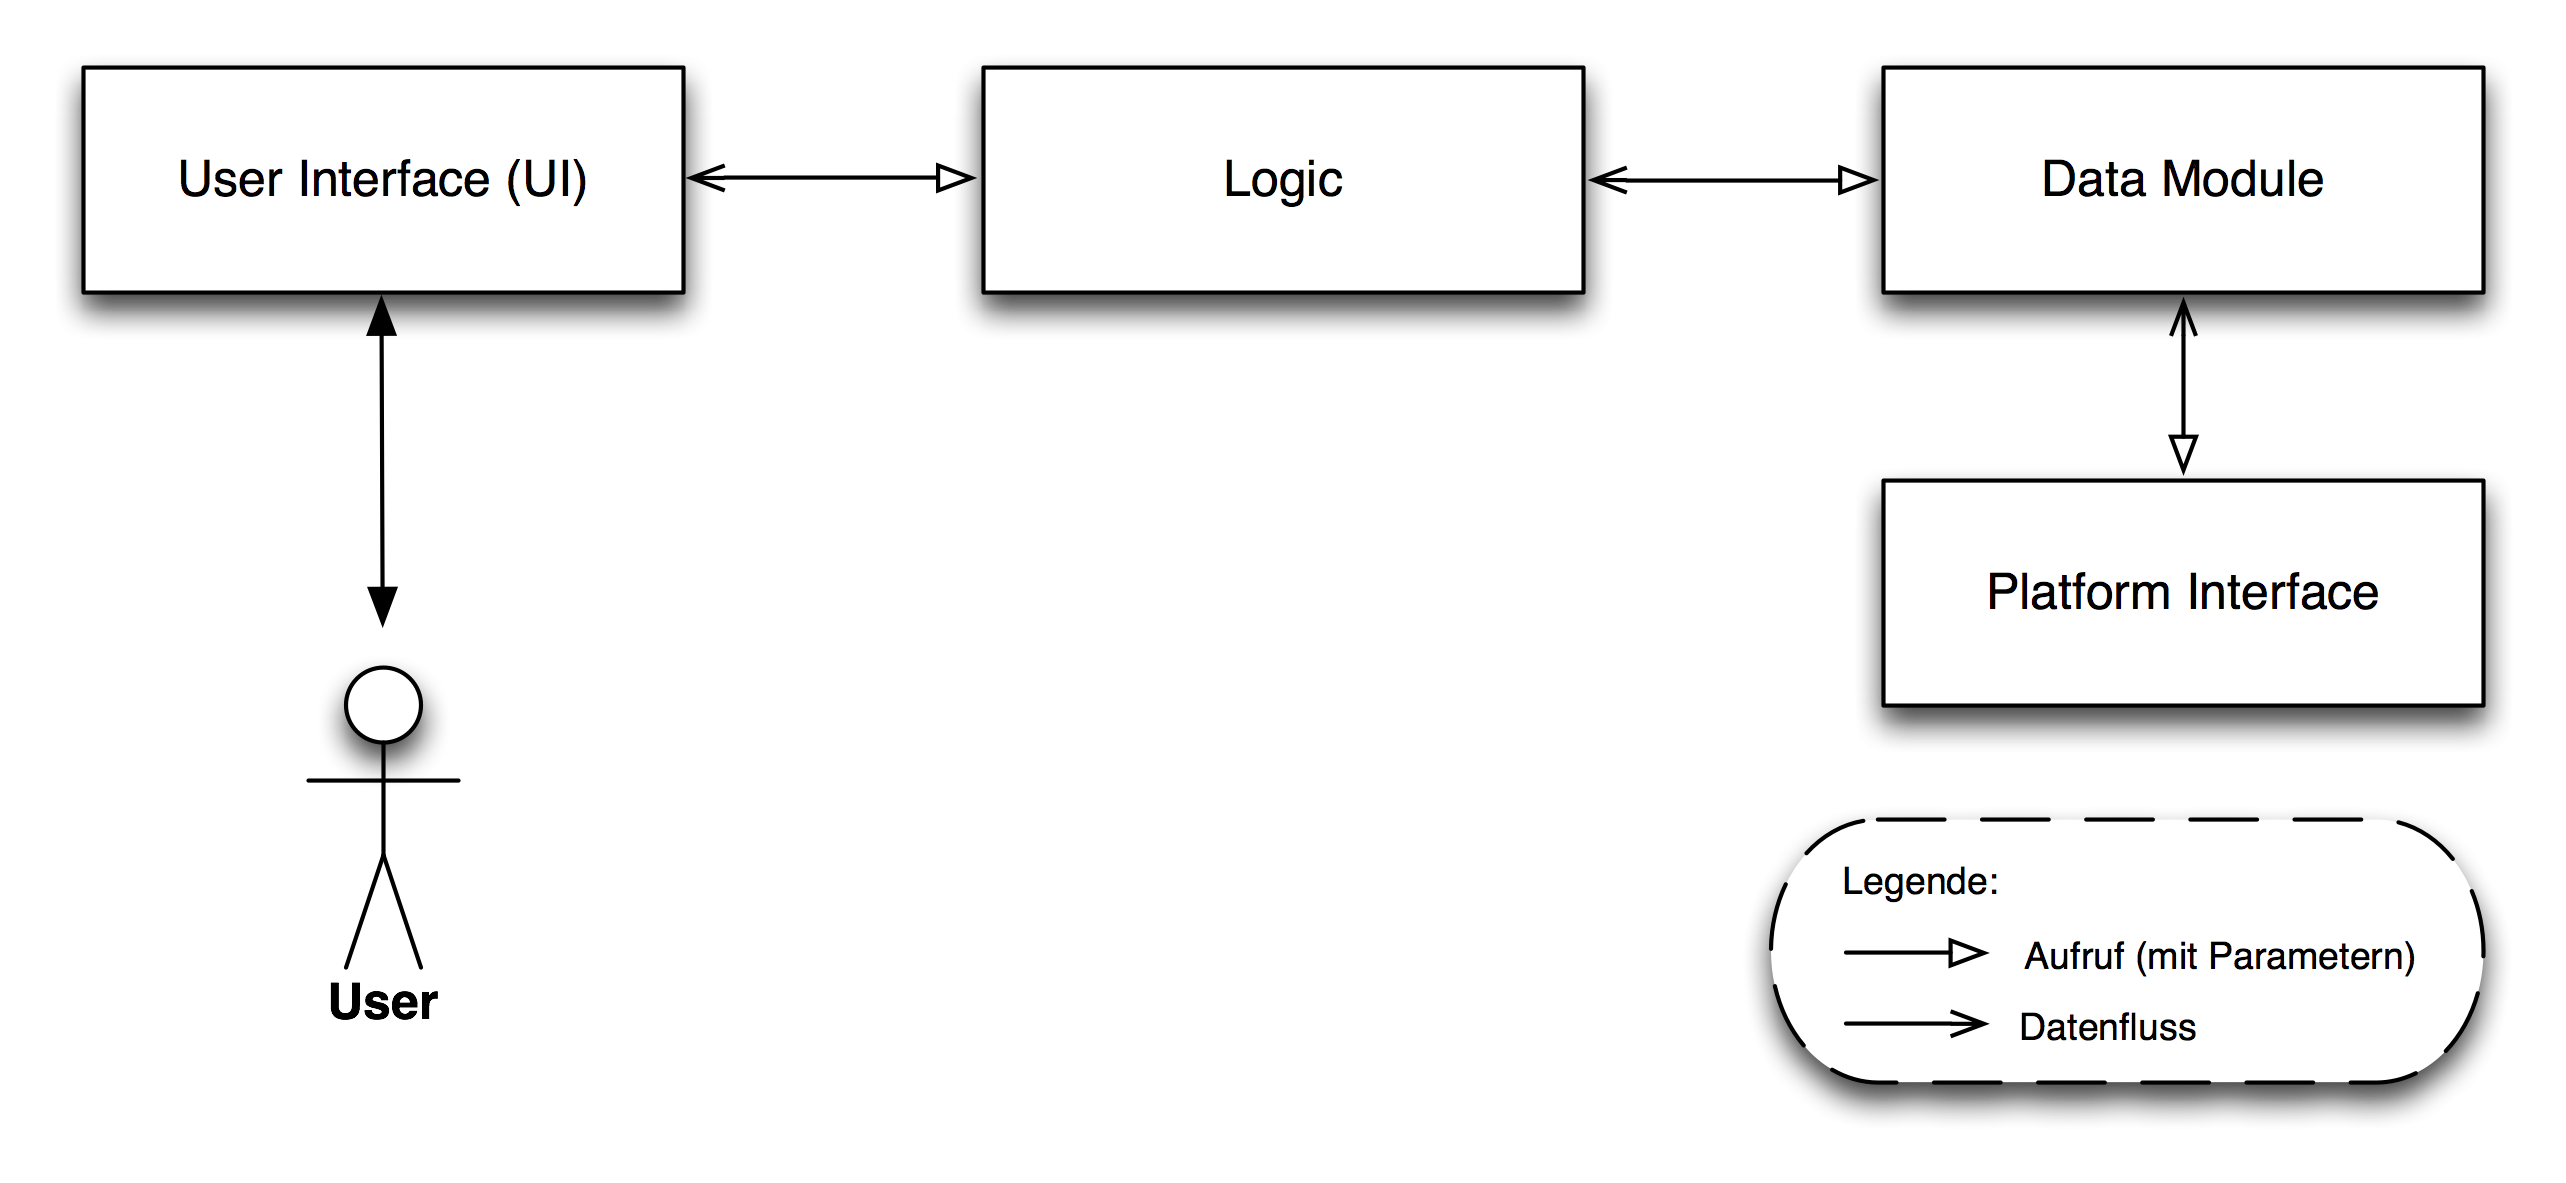
\includegraphics[width=16cm]{pics/top_level_design.png}
\caption{High level design of the system components}
\label{high_level_design}
\end{figure}

\begin{figure}[h!]
\centering
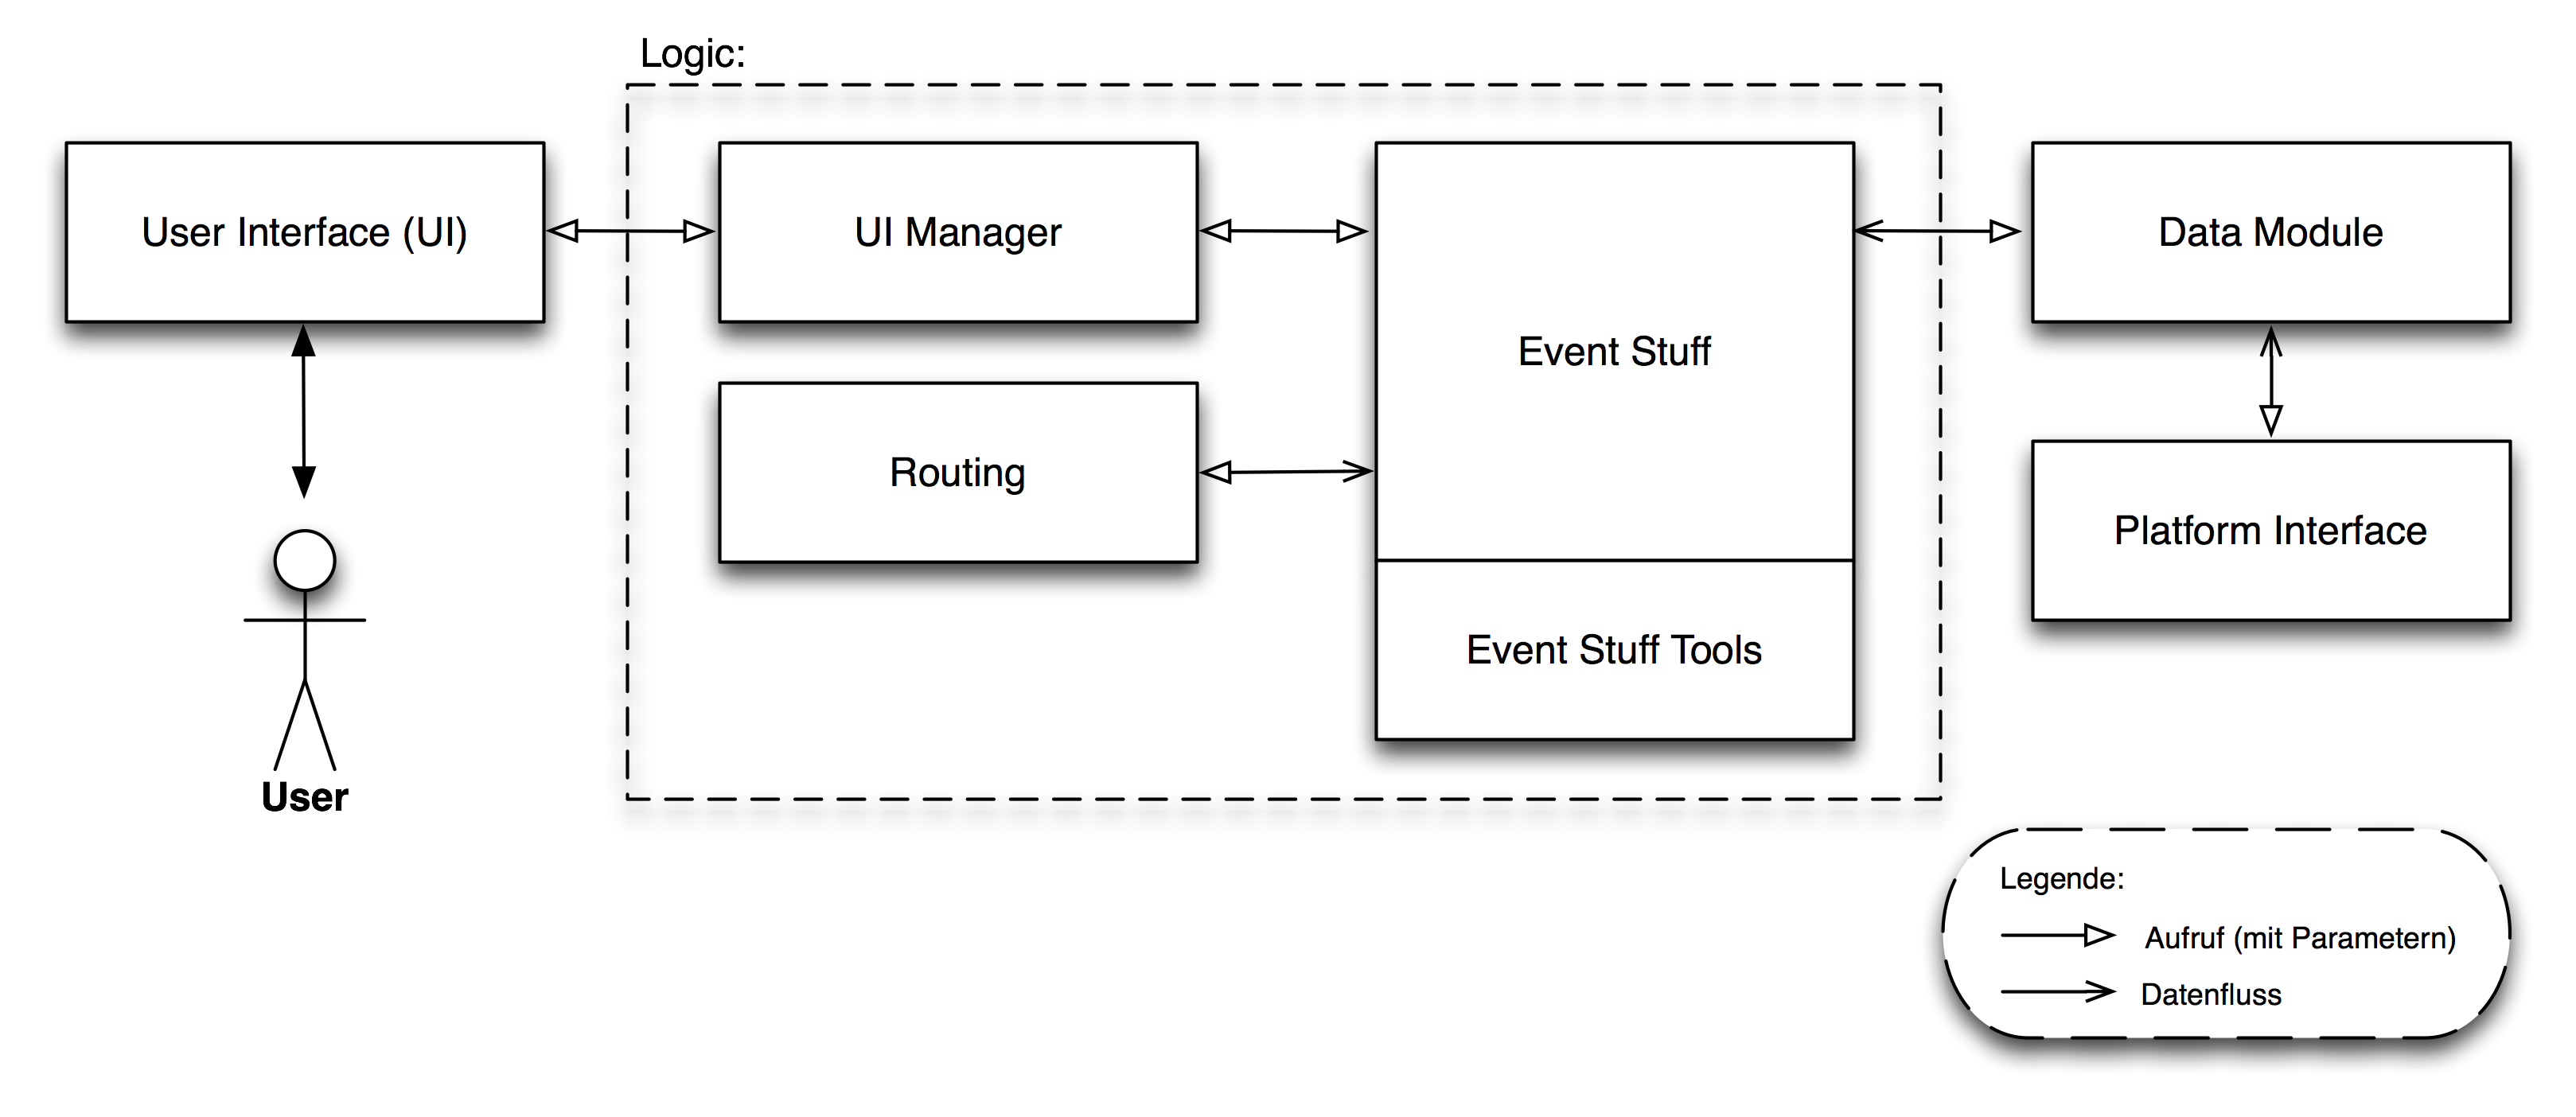
\includegraphics[width=16cm]{pics/logic.png}
\caption{Representation of the logical system elements}
\label{logic}
\end{figure}

\begin{figure}[h!]
\centering
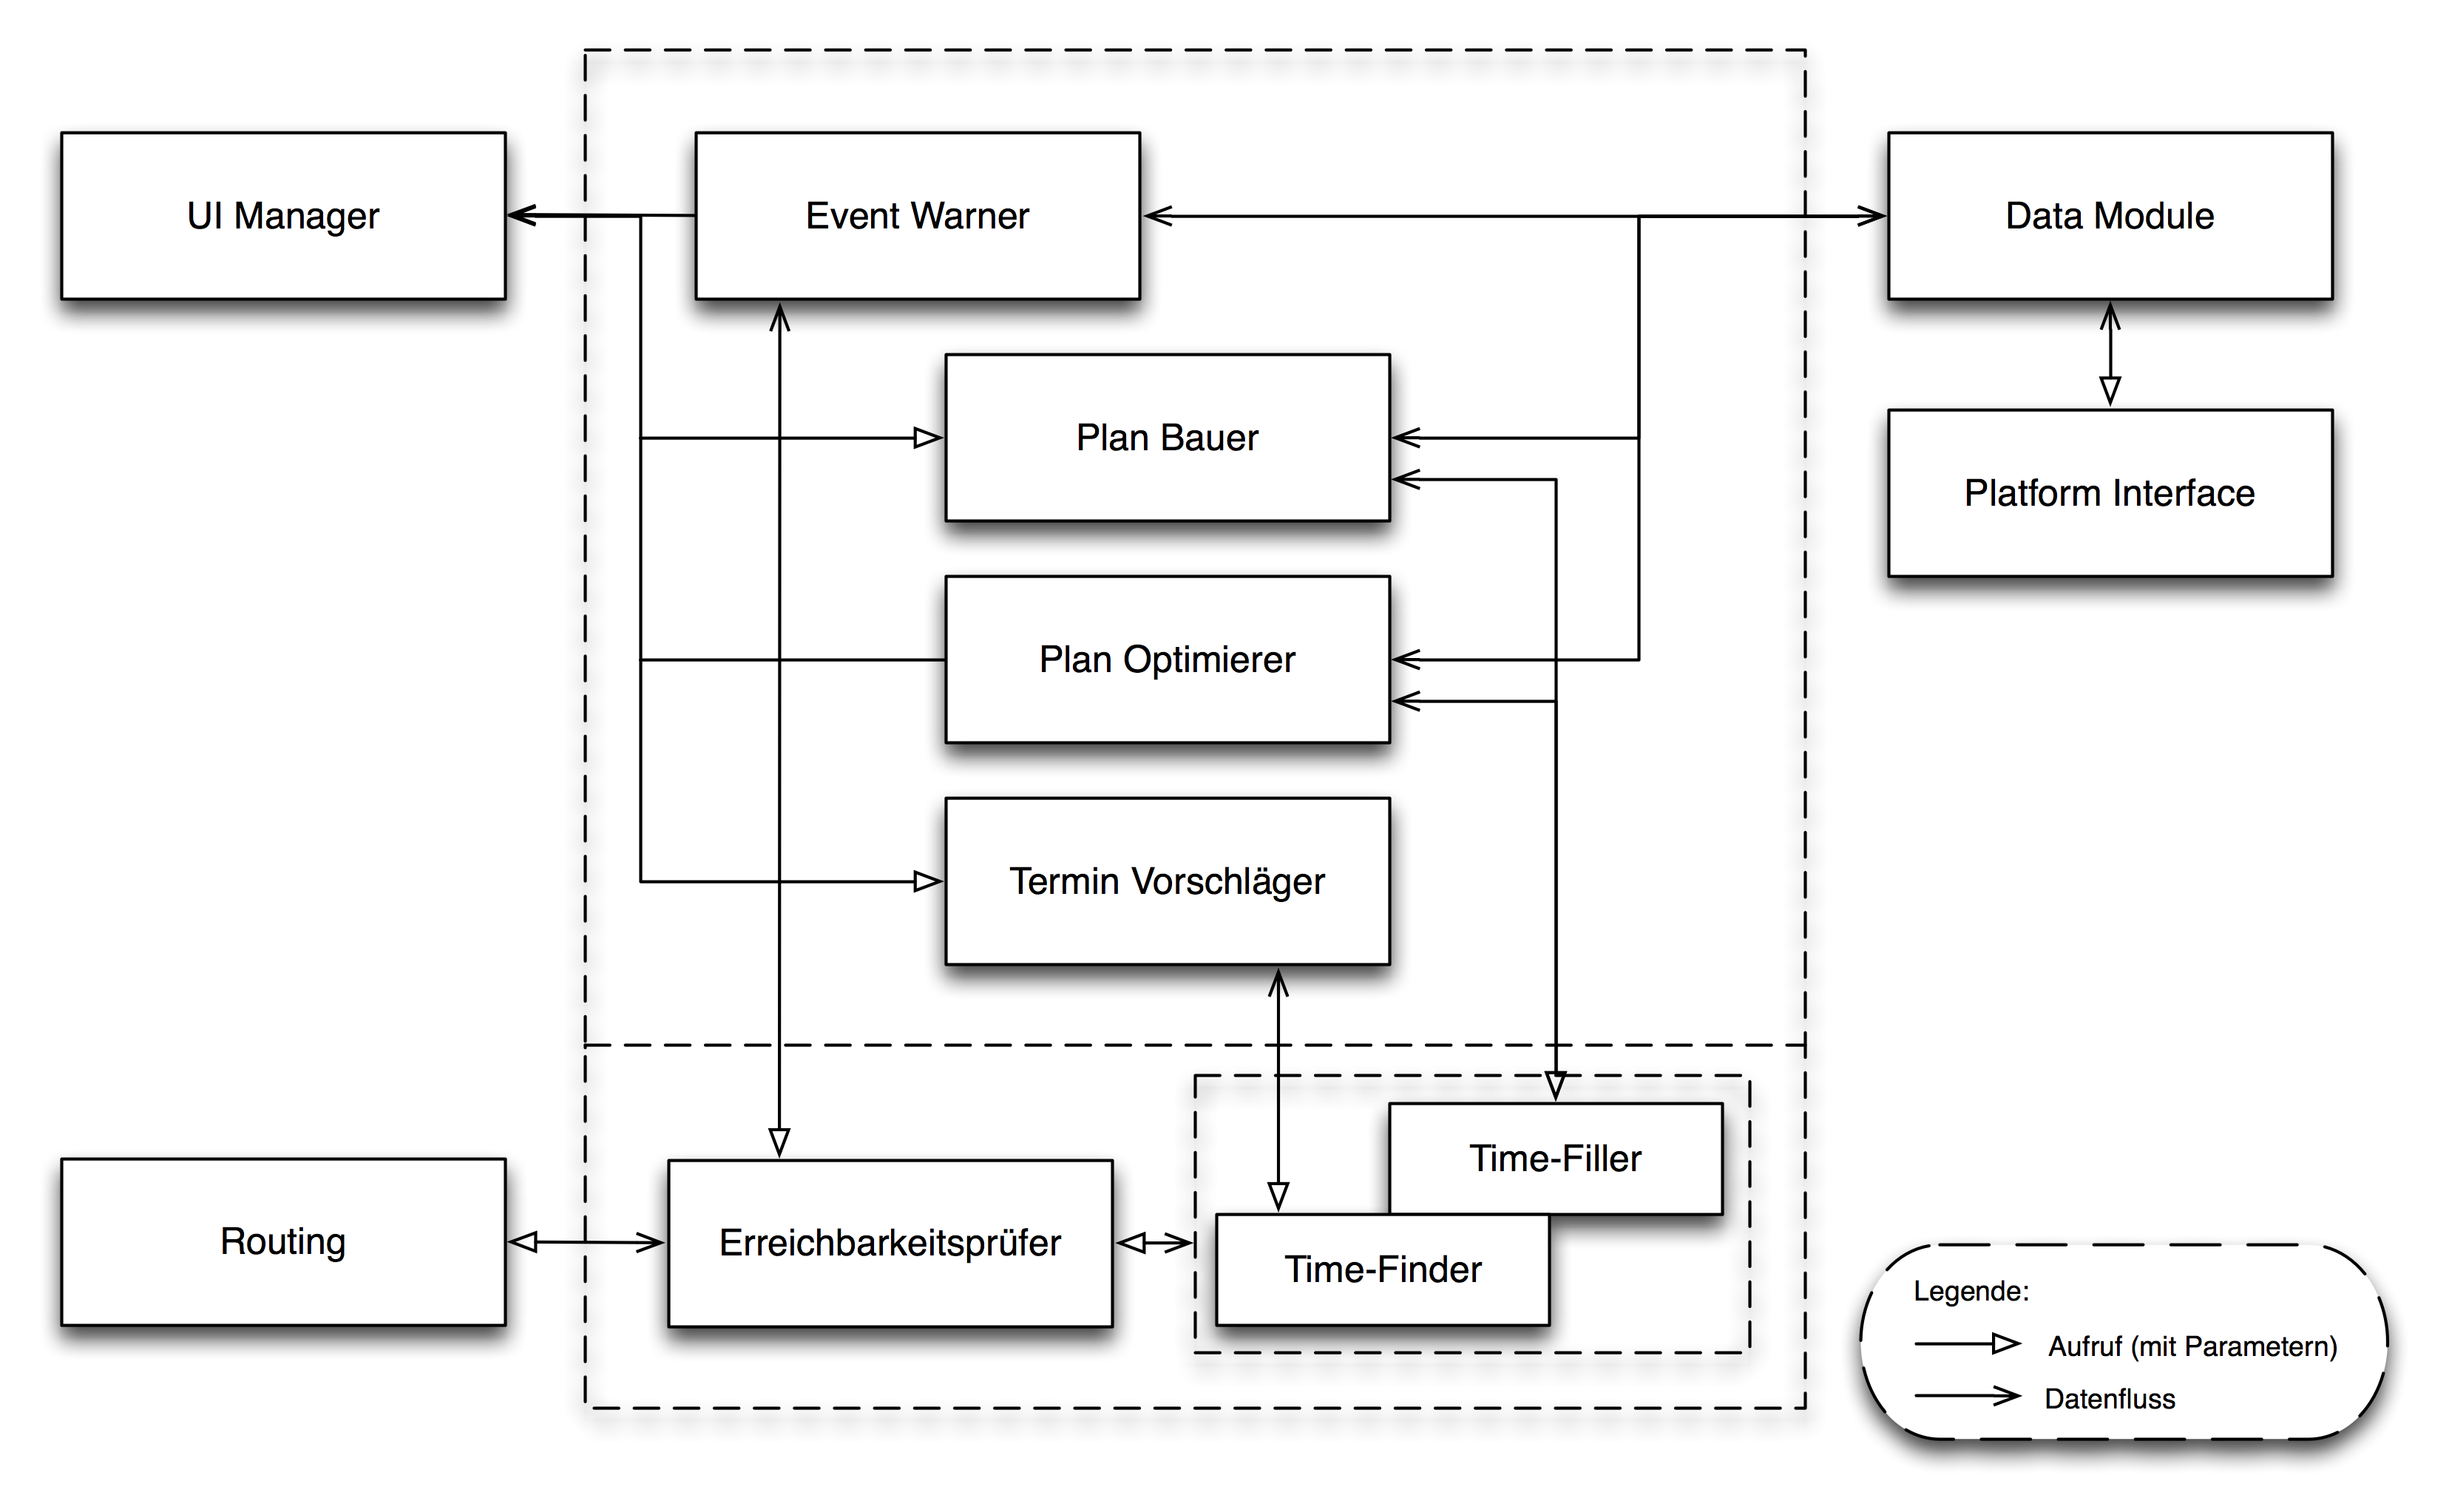
\includegraphics[width=16cm]{pics/event_stuff.png}
\caption{Components of the Appointment/Task optimization and verification engine}
\label{event_stuff}
\end{figure}

\begin{figure}[h!]
\centering
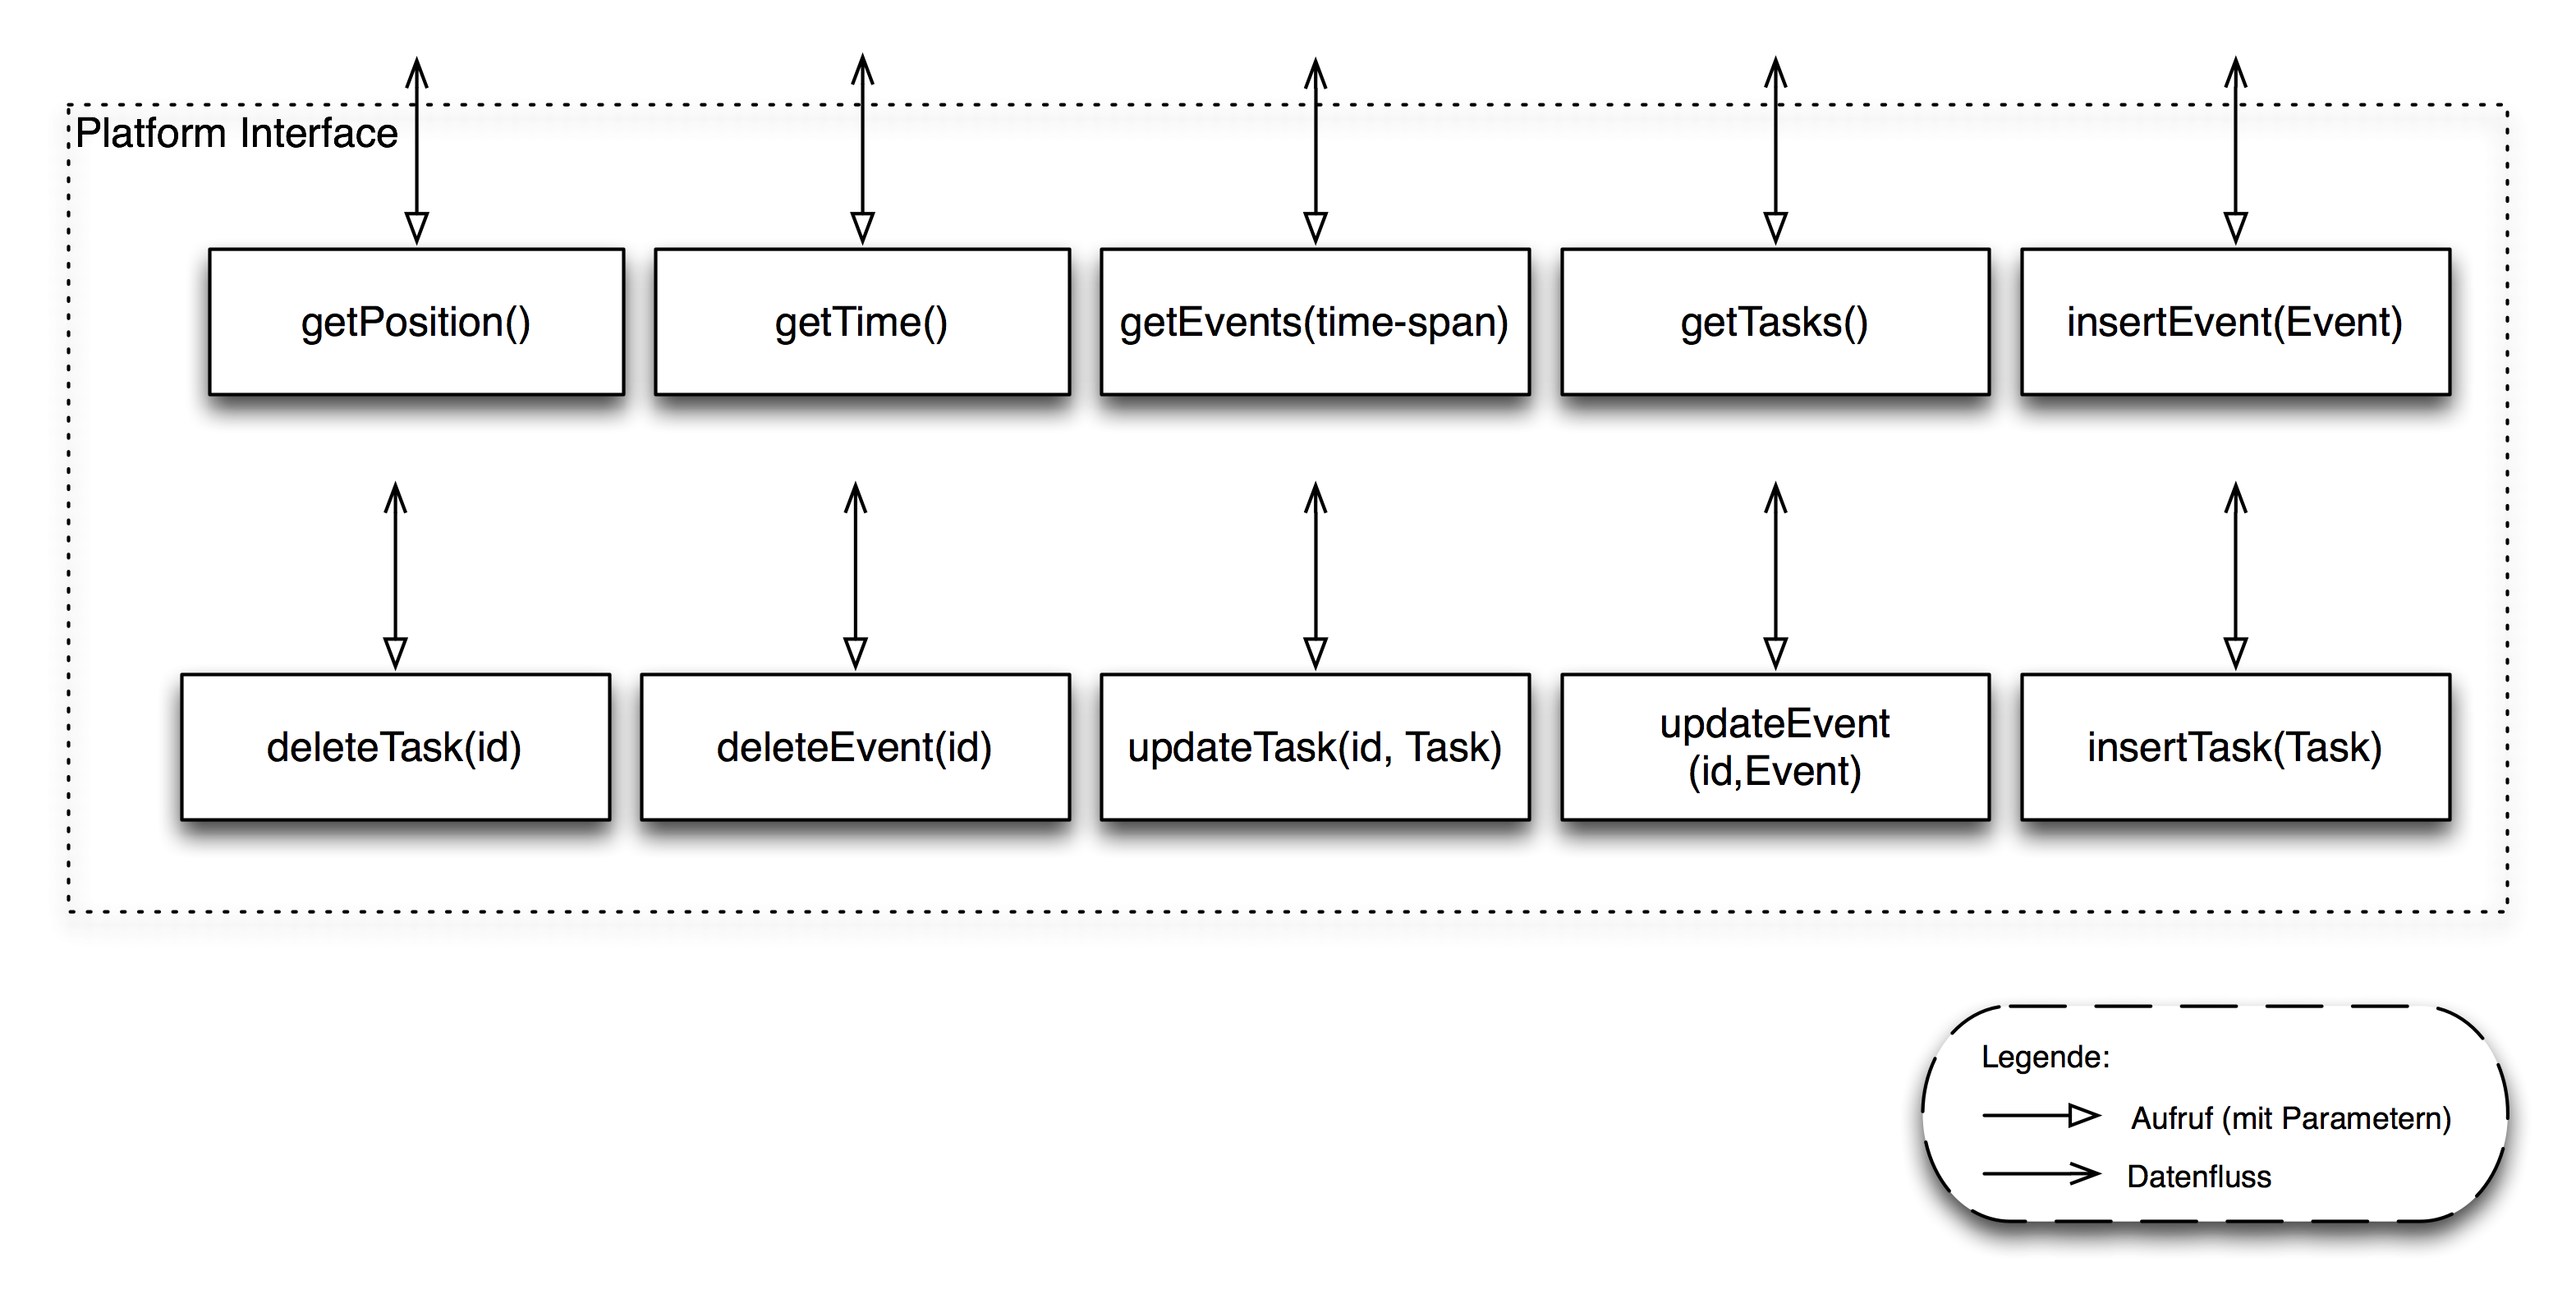
\includegraphics[width=16cm]{pics/data_module.png}
\caption{Highlevel interface for data storage and system interaction}
\label{gantt1}
\end{figure}